\section{Experimental Setup}
\label{expSetup}
The experimental setup that is described in this section, is designed to measure, the properties of LXe scintillation. However it is designed in a modular way, so it can serve different requirements from different future experiments. There are three main building blocks consisting the full setup, The purification and circulation system, the cryogenic system, and the detector system. Each building block can be replaced without effecting the others. The full assembly (figure.~\ref{fig:fulldet}) is held on three separate wracks, one for the DAQ, while the two others which hold the the detector and purification system are joined using a 100mm bar with shock absorbers on both sides.   

\subsection{Gas handling system}
\label{subsec:gas}

A typical LXe detector must keep a high level of purity. Careful selection and meticulously cleaning of all parts before mounting, is needed, however is not sufficient. The desired level of most detectors of impurity concentration is at the level of 1 ppb $O_2$ equivalent~\cite{Aprile:2009dv}. This is crucial to allow ionization electrons drift for several cm. To reach that level in a reasonable amount of time (several days instead of months), continuous purification is needed. The gas system, provides this process, alongside with all gas handling operations such as filling and recuperation.

During purification mode, xenon is taken from the chamber (in liquid phase)
passes through a heat exchanger\footnote{GEA GBS100M-24 plate heat exchanger} where it is heated and vapored. Then the xenon is forced by a KNF diaphragm pump into a hot getter\footnote{MONO-TORR
PS4-MT15-R-2} which cleans the xenon from most impurities. The xenon
also passes through an MKS Mass Flow Controller\footnote{MKS mass flow controller} (MFC). 

After the xenon is purified, it is delivered back to the cryogenic system through the heat exchanger, there the remained xenon gas is liquefied before it continuous back to the chamber. A schematic of this system is shown in fig.~\ref{fig:gasSchematic}.


\begin{figure}[t!]
\centerline{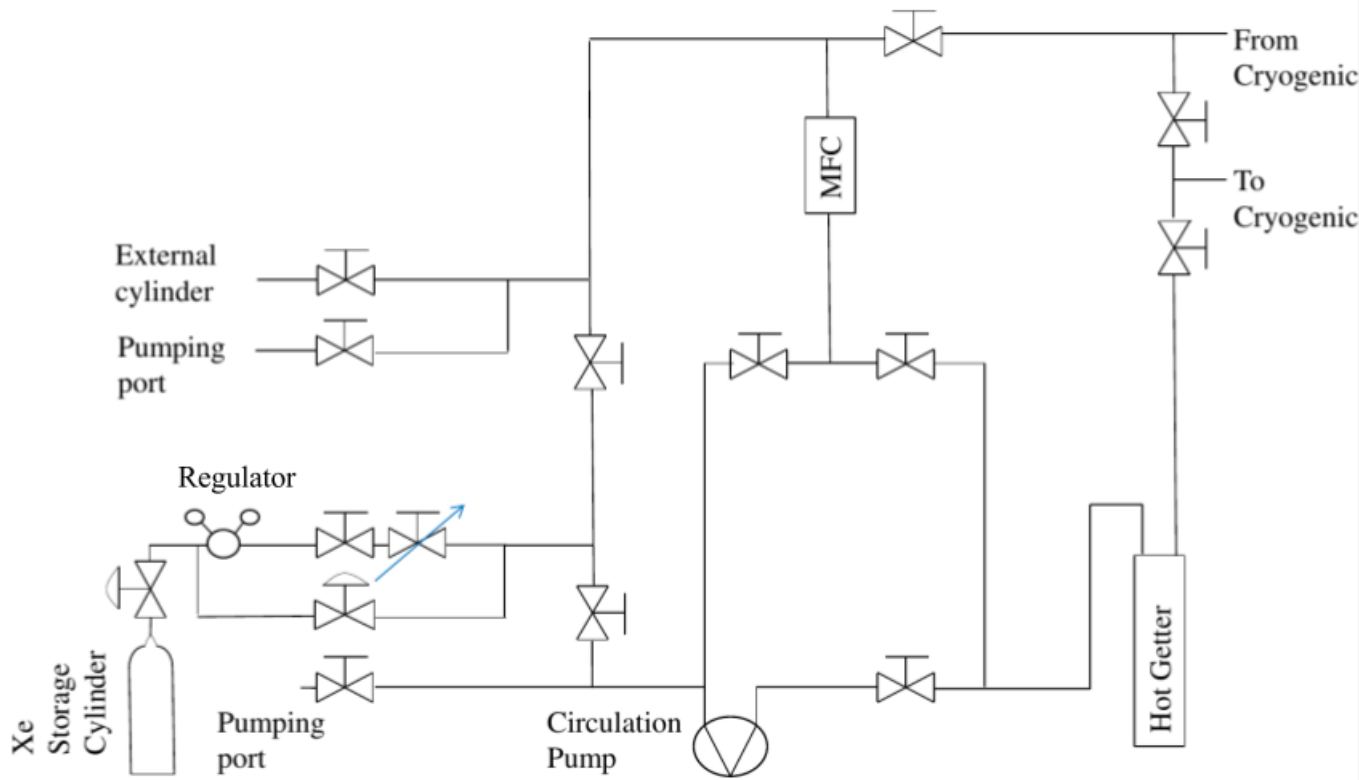
\includegraphics[width=1.\linewidth]{GasSchematics.png}}
\caption{Schematics of the purification system. High pressure valves are indicated as valves with arcs. Needle valves are indicated as a valve with an arrow.}
\label{fig:gasSchematic}
\end{figure}
\subsection{Cryogenic System}
\label{subsec:cryo}

Remote cooling is generally used in DM experiments due to background radiating from the cooler to the detector. Although in our system this is not of great importance there are still several advantages to remote cooling such as: lowering acoustic noise from the cryo-cooler and flexibility to design changes. The cryogenic system is connected on one side to the gas system and on the other to the detector chamber, any change in the system (e.g, cooler type or model) requires the change of that specific part without changing the detector nor the gas system.

The system is made out of two chambers, the outer vessel (OV) which holds the insulation vacuum, and the inner vessel (IV) that holds the xenon. In addition to the vacuum which prevents heat leaks from diffusion and convection, the entire IV is covered by multi layer aluminized Myler to prevent heating via radiation A picture of the detector and the CAD design are shown in Fig~\ref{fig:cryo}. 
\begin{figure}
   \centering
    \begin{subfigure}[b]{0.25\textheight}
    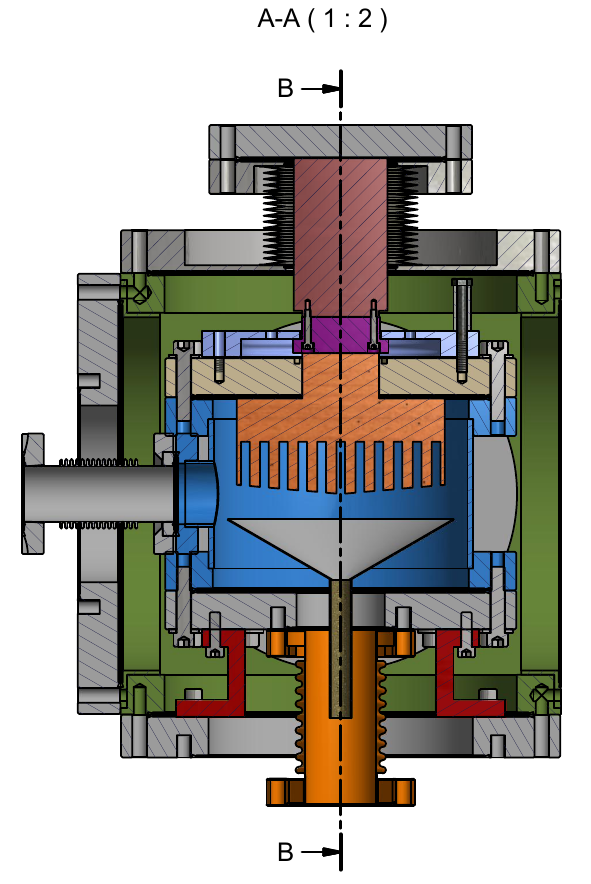
\includegraphics[width=\textwidth]{cryogenic1.png}
    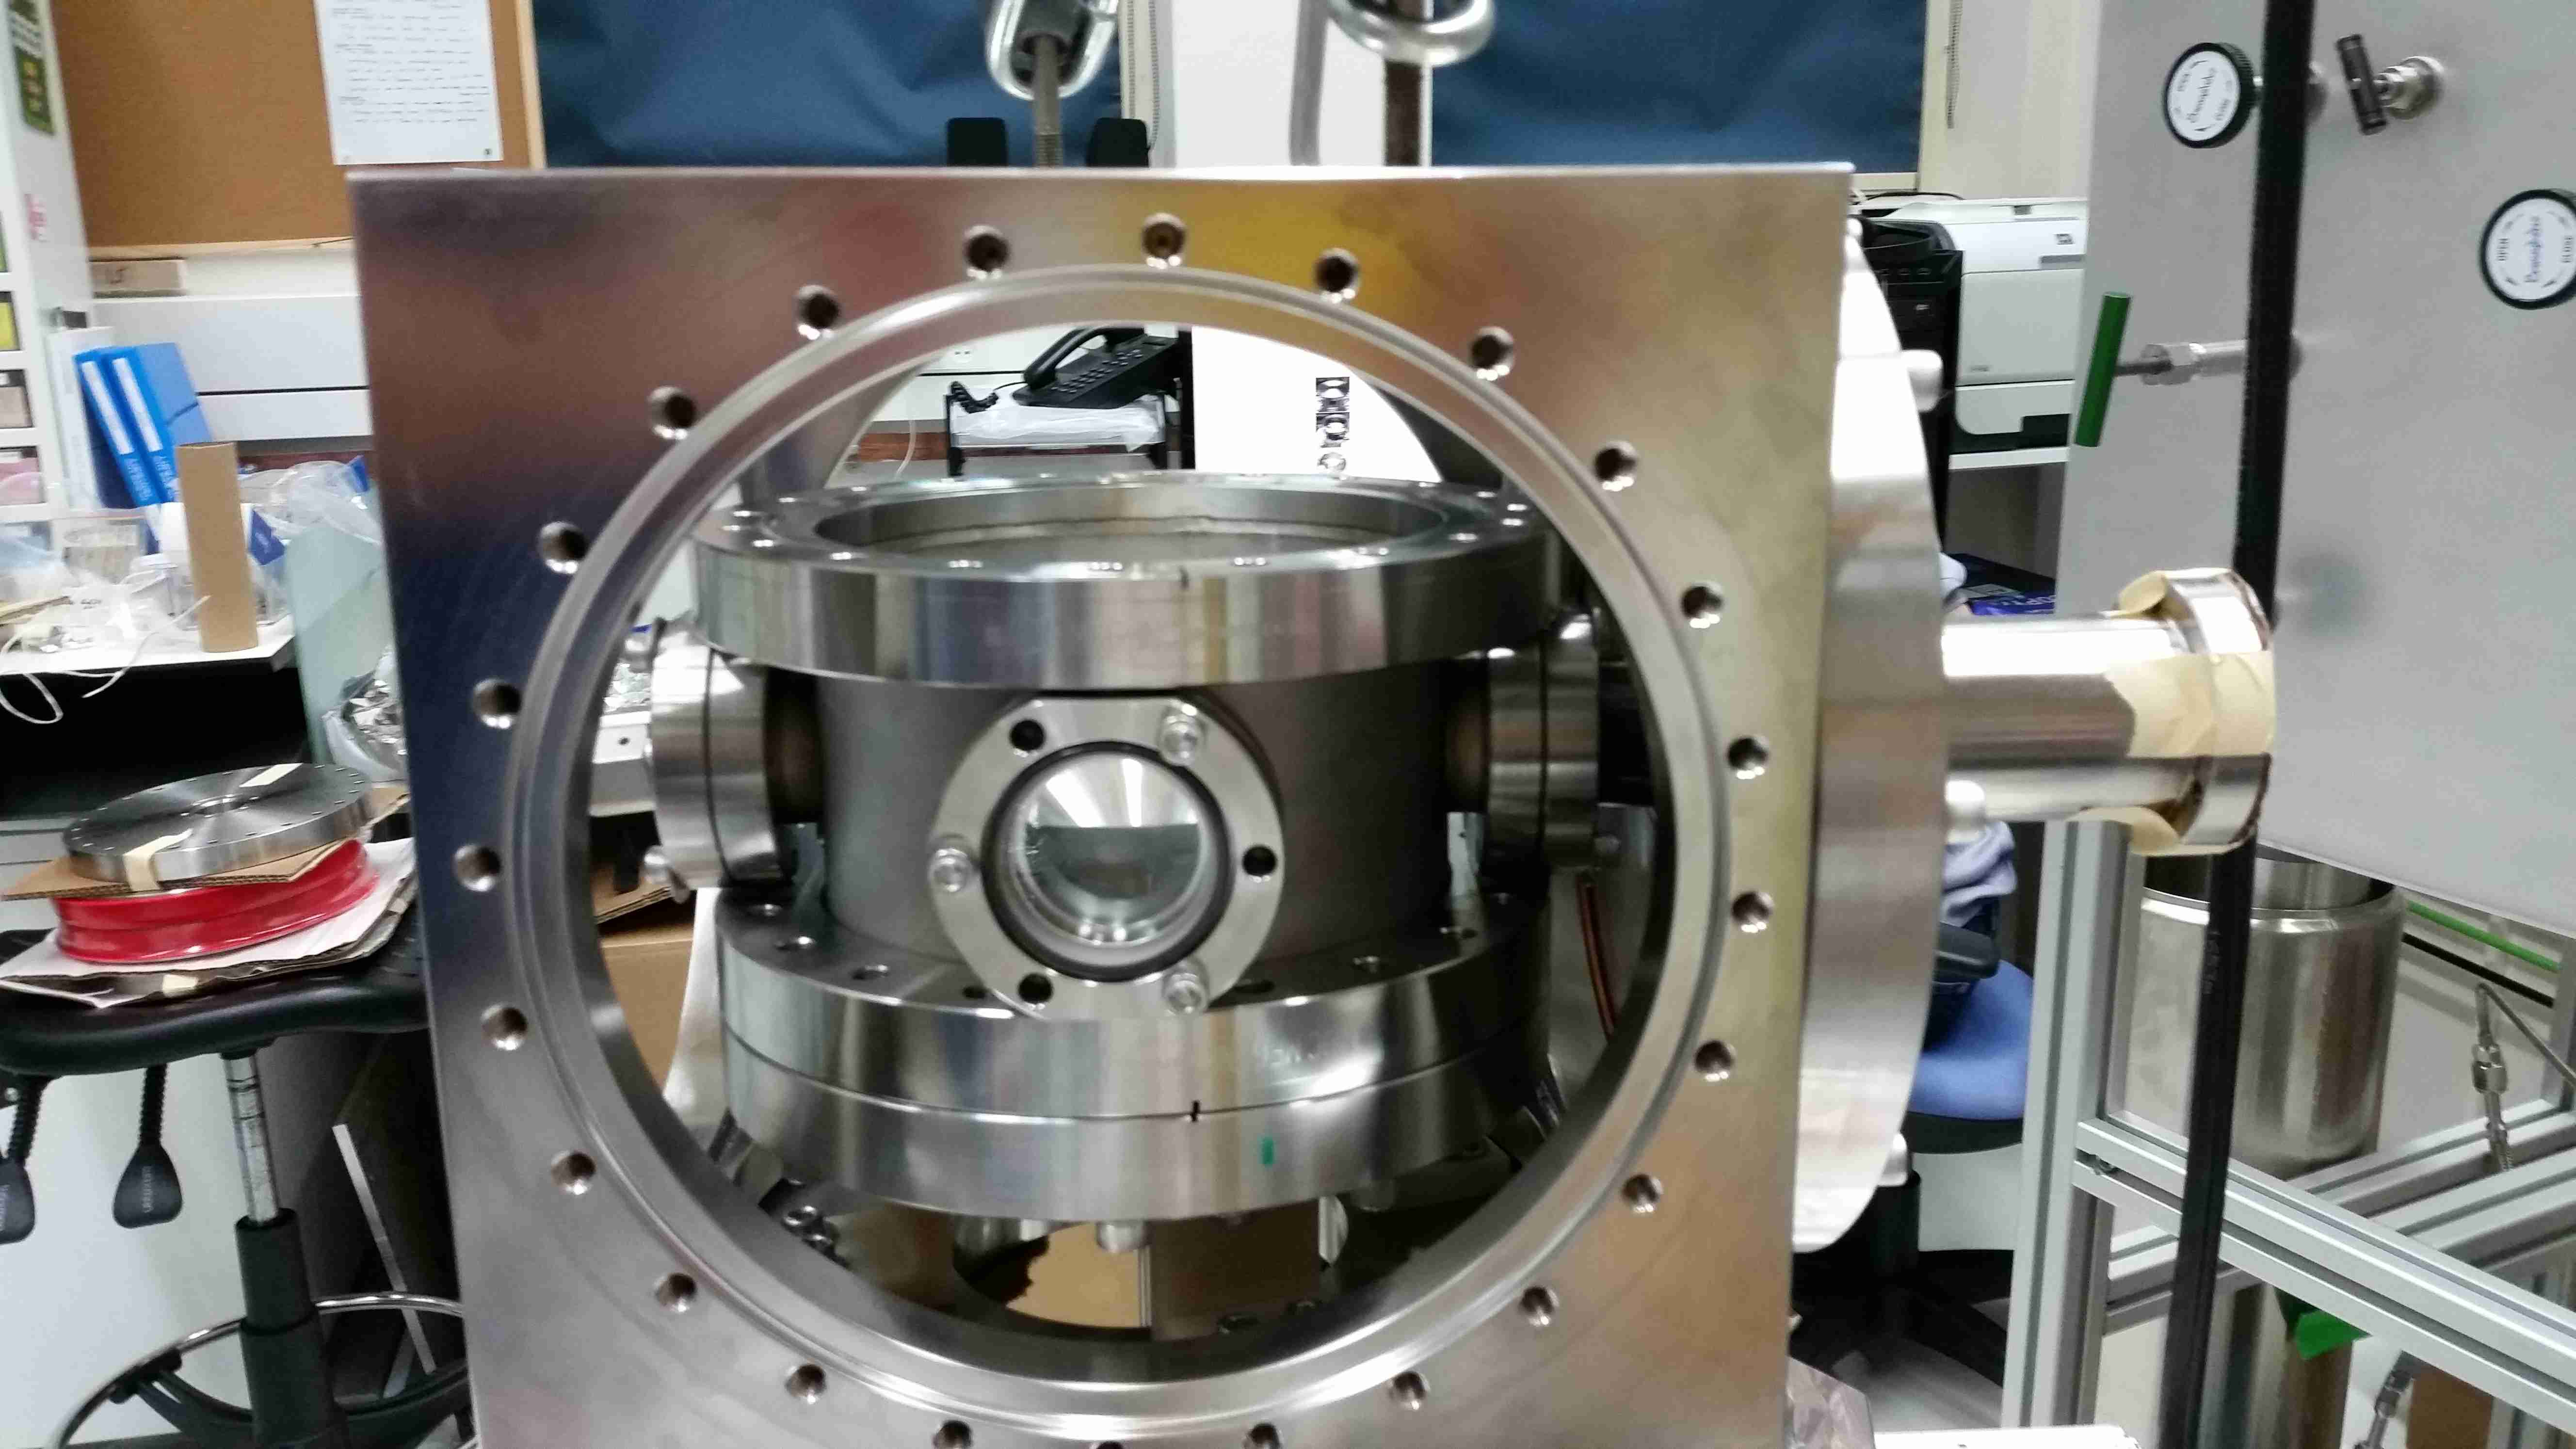
\includegraphics[width=\textwidth]{CryoOpen_small.jpg}
    \end{subfigure}
        \caption{(Top) CAD view of the cryogenic system. (Bottom) Pictue of the cryogenic system. \label{fig:cryo}}
\end{figure}


The OV is made of a 10" CF cube, with ports on all six faces (e.g., FT, pumping ports, view ports). The space between the OV and IV is held in vacuum for heat insulation (convection and diffusion). This vacuum is shared with the detector one via a 6" CF flexible bellows.

The IV is made of XXX~\,cm height cylinder with 6" CF flanges on the top and bottom parts of it, and it holds inside xenon. A XXX~" cold finger is welded to the top flange of the IV. The design of the cold finger is similar to the design of~\cite{xe100_instr2012}, the inner part of the cold finger is made of long fins, therefore the surface area of it is bigger resulting in a better heat transport. The upper part of the cold finger is in thermal contact with the cryo-cooler~\footnote{QDrive 20BB 9p6 A 3 AYNBNCO} via a cooper adapter. The copper adapter hold two $100\Omega$ pt resistor which are connected to a PID reader\footnote{cryo-con model 18i Cryogenic Temp Monitor} fot temperature measurements. A Cartridge-heater is also inserted to the copper adapter for emergency heating. 

The cryo-cooler provides up to 70 W of cooling power,and is connected via a 4 1/2" flange to the OV top flange, and reaching the IV top flange. Common cryo-coolers used for xenon experiments, work in maximal cooling mode permanently. The QDrive, instead, has temperature control allowing it vary the cooling power, which enables to set the temperature with fluctuations smaller then $0.1~\mathrm{C^{\circ}}$ on the cooler itself.

On the inner side of the bottom flange of the IV a thin SS funnel is installed collecting all LXe drops from the cold finger, and delivering them to the  detector part. This flange is connected to the detector part, via a 3 3/8" flexible bellows. This bellows hosts two small pipes connected to the circulation system, and a third pipe coming from the funnel, all three pipes deliver LXe whereas the GXe is filling the bellows.

      


\subsection{The Detector}
\label{subsec:det}
